\chapter{Albero di copertura minimo (MST)}

{Sia $T$ un albero di copertura,definisco}

$w(T) = \sum_{(u,v)\in T}{w(u,v)}$

{dove $w:E\rightarrow \mathbb{R}$ è detta ``funzione peso''}

{Definizione:}

{Un albero di copertura }$T${~si dice minimo o ``di peso minimo'' (minimum spanning tree) se $w(T)$ è il minimo rispetto a tutti gli alberi di copertura}

\subsection{Teorema fondamentale degli MST}

{Sia $G=(V,E) [NO]$ connesso con funzione peso $w$.}

{Se le tre condizioni}

\begin{enumerate}
\tightlist
\item
  {$A \subseteq E$ è contenuto in qualche MST}
\item
  {$(S,V \setminus S)$ è un taglio che rispetta $A$}
\item
  {Sia $(u,v)$ un arco leggero che attraversa il taglio $(S,V \setminus S)$}
\end{enumerate}

{sono rispettate, allora l'arco $(u,v)$ è sicuro per $A$, ovvero $A \subseteq \{(u,v)\}$ è contenuto in qualche MST.}

\subsubsection{Dimostrazione}

{$A \subseteq T$ con $T$ MST}

{Due casi:}

\begin{enumerate}
\tightlist
\item
  {$(u,v) \in T$, caso banale in quanto $A \cup \{(u,v)\} \subseteq T$  e $T$ è l'MST che cerchiamo.}
\item
  {$(u,v) \notin T$, quindi $T$ non è l'MST che cerchiamo, procediamo quindi a costruirne uno:}
\end{enumerate}

{Per le sei proprietà fornite, se unisco $(u,v)$ a $T$ formo un ciclo, è quindi necessario rimuovere l'altro cammino $(x,y)$ che lo forma tra gli archi che attraversano il taglio. }

$T' = T \cup {(u,v)} \setminus \{(x,y)\} $

\begin{figure}[H]
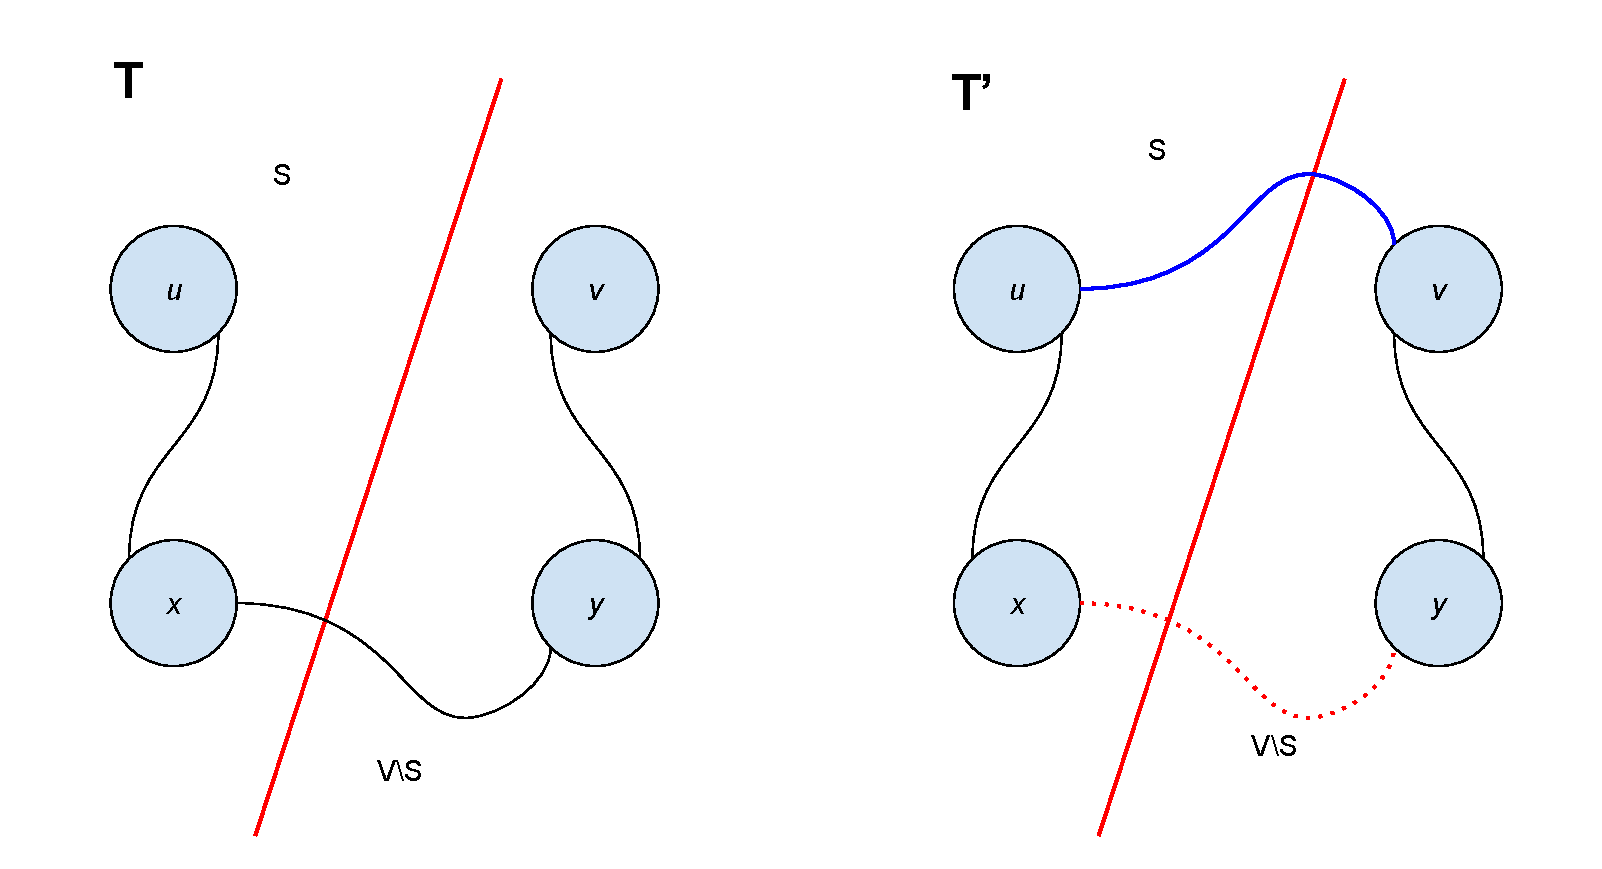
\includegraphics{graphs/arco_taglio_leggero.pdf}
\end{figure}

$w(u,v) \leq w(x,y)${: Il peso dell'arco aggiunto è minore del peso dell'arco rimosso, in quanto esso è leggero per ipotesi.}

{Quanto vale allora $w(T')$? }

$w(T') \leq w(T)$ {ed essendo }$w(u,v) \leq w(x,y)${~allora $w(T') \leq w(T)$}

{Da }$w(T) \leq w(T') \leq w(T)$ \textsuperscript{\protect\hyperlink{cmnt26}{{[}z{]}}}{risulta che $w(T') = w(T)$, e }$T'${~è quindi un MST.}

{Nota}\textsuperscript{\protect\hyperlink{cmnt27}{{[}aa{]}}}{: se $w(u,v) = w(x,y)$ allora $(u,v) = (x,y)$?}

{Dobbiamo però dimostrare che $T'$ sia ``sicuro'', e perciò dimostriamo che \\ $A \cup \{(u,v)\} \subseteq T'$}

\subsection{Corollario}

{Sia $G=(V,E) [NO]$ connesso con funzione peso $w$. Se le tre condizioni}

\begin{enumerate}
\tightlist
\item
  {$A \subseteq E$ è contenuto in qualche MST}
\item
  {$C$ è una componente connessa della foresta $(V,A)$}
\item
  {Sia $(u,v)$ un arco leggero che collega la componente $C$ con il resto del grafo}
\end{enumerate}

{sono rispettate, allora l'arco $(u,v)$ è sicuro per $A$, ovvero $A \cup \{(u,v)\}$ è contenuto in qualche MST.}

\subsubsection{Dimostrazione}

{Se impongo che}

\begin{itemize}
\tightlist
\item
  {Il taglio dell'ipotesi 2 sia $(C,V\setminus C)$, in modo da isolare la componente connessa}
\item
  {MANCA}\textsuperscript{\protect\hyperlink{cmnt28}{{[}ab{]}}}
\end{itemize}

{posso utilizzare il teorema fondamentale per la dimostrazione}

\subsection{Corollario}

{Sia $(u,v)$ un arco di peso minimo in $G$. Allora $(u,v)$ appartiene a qualche MST.}

\subsubsection{Dimostrazione tramite la tecnica ``cuci e taglia''}

{Sia T un MST di G. }

{Due casi:}

\begin{enumerate}
\tightlist
\item
  $(u,v)\in T${, ovvio}
\item
  $(u,v)\notin T$
\end{enumerate}

\subsection{Corollario}

{Sia $(u,v)$ un arco di peso minimo in $G$ e supponiamo che sia unico. Allora $(u,v)$ appartiene a tutti gli MST}\textsuperscript{\protect\hyperlink{cmnt29}{{[}ac{]}}}{.}

\subsubsection{Dimostrazione per assurdo}

{Nonostante le ipotesi, esiste {[}almeno{]} un MST senza l'arco in
questione.}

{Non esistendo, provvediamo ad aggiungerlo a T. $T' = T \cup \{(u,v)\}$}

{Facendo ciò creo sicuramente un ciclo, in quanto $T$ è albero. Scelto un arco $(x,y)$ e lo rimuovo. Ho quindi costruito un albero di copertura con peso $W(T') = W(T) + w(u,v) - w(x,y) < W(T)$}

{Con $w(u,v) < w(x,y)$ (minore stretto!)}

{Contraddizione}{: essendo T MST, non può esistere un altro albero con peso inferiore.}

\subsection{Esercizio}

$G=(V,E) [NO]$ connesso con $w:E \rightarrow \mathbb{R}$

{Sia $T_{min}$ un MST di G.}

{Sia $T'$ un albero di copertura (ST) non necessariamente minimo (M).}

{Siano $(u,v),(x,y)$ rispettivamente gli archi di $T,T'$ di peso massimo. Ordino gli archi e considero i pesi maggiori.}

$T_{min}: <e_1,e_2,\ldots,e_{n-1}>$ con $e_{n-1} = (u,v)$

$T': <e'_1,e'_2,\ldots,e'_{n-1}>$ con $e'_{n-1} = (x,y)$

{Congettura: $w(u,v) \leq w(x,y)$}

{Si può procedere per confutazione con controesempio oppure per dimostrazione tramite metodo ``cuci e taglia''.}

{Soluzione}\textsuperscript{\protect\hyperlink{cmnt30}{{[}ad{]}}}{:}

\subsection{Esercizio}

{Dimostrare che, se tutti i pesi del grafo sono distinti, allora esiste un solo MST.}

{Soluzione}\textsuperscript{\protect\hyperlink{cmnt31}{{[}ae{]}}}{:}

\subsubsection{Generazione degli alberi di copertura minima}

\lstinputlisting{code/generic_mst.txt}

{Verranno analizzati gli algoritmi di Kruskal e Prim, i quali differiscono per l'implementazione della ricerca dell'arco sicuro.}

{Kruskall utilizza le strutture dati Set per la gestione di insiemi disgiunti. Esse dispongono di tre operatori:}

\begin{enumerate}
\tightlist
\item
  {Make\_set(X)}
\item
  {Union(x,y) o Merge\_set(x,y)}
\item
  {Find\_set(x)}
\end{enumerate}

{Esempio di utilizzo: determinare le componenti connesse di un grafo}

\lstinputlisting{code/componenti_connesse.txt}

\subsubsection{Generazione di MST : Kruskal}

$G=(V,E)$ connesso, $n=\abs{V},m=\abs{E}$

\lstinputlisting{code/kruskal.txt}

{*Per l'analisi delle due find\_set e della union ci viene fornita la complessità ottenuta tramite Heichmann.\\
}{Complessità}{:}

{$O(mlog(m)+n+mlog(m))$, avendo $m \geq n-1$ archi poichè l'arco è connesso, la complessità è $O(mlog(m))$}

\subsubsection{Simulazione di esecuzione}

\subsubsection{Tramite grafo}

%{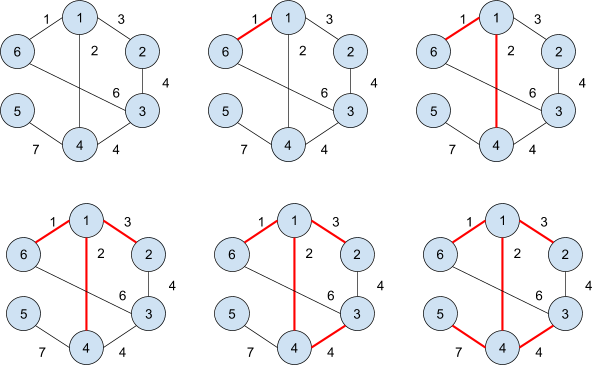
\includegraphics{images/image519.png}}
\begin{figure}[H]
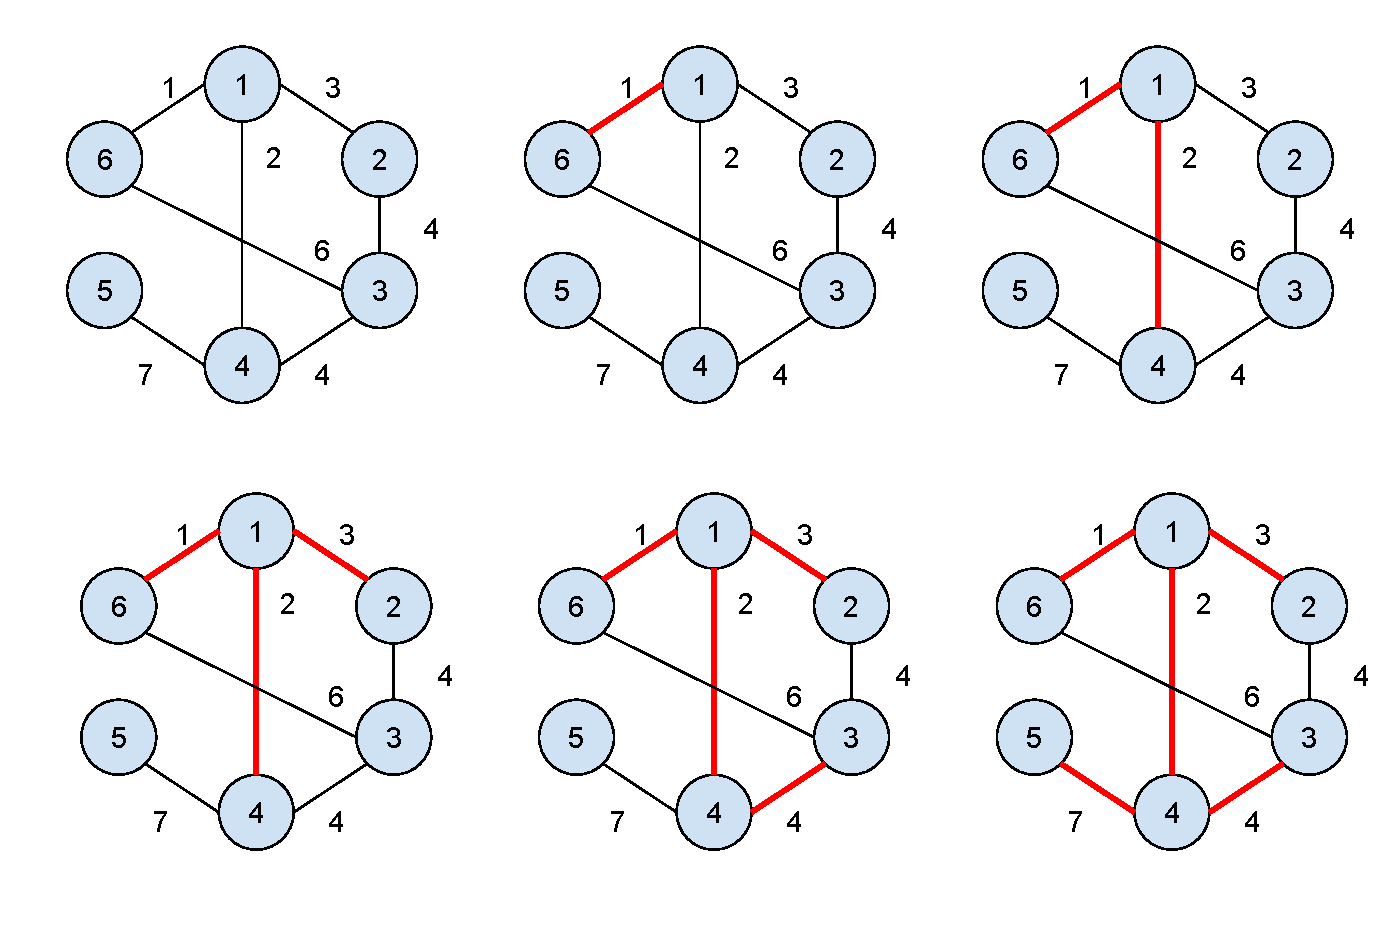
\includegraphics{graphs/simulazione_grafo.pdf}
\end{figure}


\subsubsection{Tramite tabella}

\begin{tabular}{|l|l|l|}
\hline 
Passo & A & Insiemi disgiunti \\ 
\hline 
1 & $\{\}$ & $\{1\},\{2\},\{3\},\{4\},\{5\},\{6\}$ \\ 
\hline 
2 & $\{(1,6)\}$ & $\{1,6\},\{2\},\{3\},\{4\},\{5\}$ \\ 
\hline 
3 & $\{(1,6),(1,4)\}$ & $\{1,4,6\},\{2\},\{3\},\{5\}$ \\ 
\hline 
4 & $\{(1,6),(1,4),(1,2)\}$ & $\{1,2,4,6\},\{3\},\{5\}$ \\ 
\hline 
5 & $\{(1,6),(1,4),(1,2),(4,3)\}$ & $\{1,2,3,4,6\},\{5\}$ \\ 
\hline 
6 & $\{(1,6),(1,4),(1,2),(4,3),(4,5)\}$ & $\{1,2,3,4,5,6\}$ \\ 
\hline 
\end{tabular} 

\subsubsection{Generazione di MST : Prim}

{A differenza di Kruskal, Prim richiede un vertice di partenza detto ``radice''. Con l'insieme Q si indica l'insieme dei vertici da estrarre.
$V\setminus Q$ indica quindi l'insieme dei vertici già estratti. $Q$ è una coda di priorità, implementata tramite Heap Binario, i cui elementi hanno le seguenti caratteristiche:}

\begin{itemize}
\tightlist
\item
  Predecessore: $\pi[u]$
\item
Chiave: $Key[u]$ valore dell'arco incidente che attraversa il taglio $(Q,Vsetminus Q)$ con peso minore. Si utilizza il valore infinito positivo per indicare l'eventuale assenza di archi.
\end{itemize}

\lstinputlisting{code/prim.txt}

La convergenza risulta essere finita

La complessità della funzione Prim è $O(m logn)$

{Simulazione}

{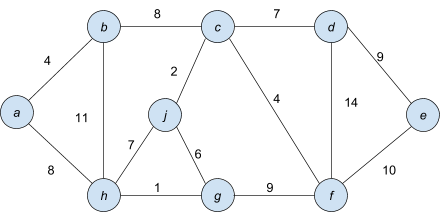
\includegraphics{images/image542.png}}
